\chapter{Implementation}
\renewcommand{\baselinestretch}{\mystretch}
\label{chap:implementation}

\begin{figure}[h!]
  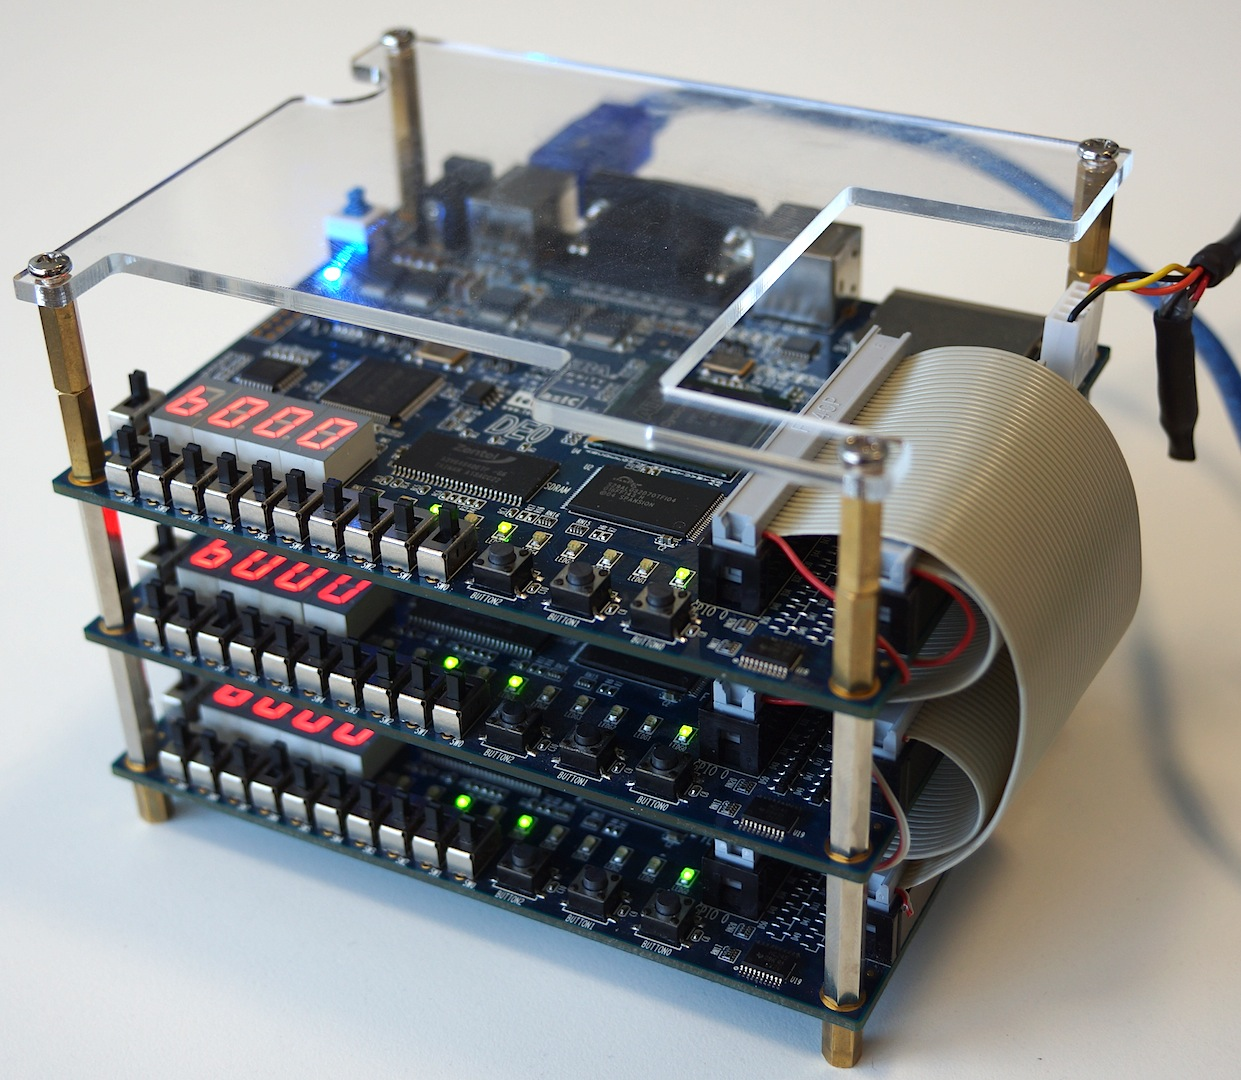
\includegraphics[width=\textwidth]{./figs/cluster.jpg}
  \caption{Hardware Implementation}
  \label{fig:cluster}
\end{figure}
%\setlength{\parindent}{0pt}
As discussed in the design section, one of the main features of this design was organising the processors to run in lockstep. This meant there were no internal data transfer protocols other than simple ready/available data signals. As a result the vast majority of the design translated from simulation to device implementation in a straight forward way. The only non-deterministic element of the design was the shared clock across multiple devices, this element required some simple analysis to identify the limits. The clock frequency needs fine control in order to limit the error rates in the data transfer. This was done by using a phase locked loop (PLL) on the master device, this takes the local 50~MHz clock as an input and outputs a compile time set frequency. This clock is then put out across 1 GPIO pin. As described in the design section this is then used as the clock input of all the devices. 

The clock frequency maximum set by the on board logic was 31MHz, ideally the inter-FPGA communication also fits this limit, allowing maximum speed of operation. The velocity of propagation for the ribbon cable is 4.53~nsM${^{-1}}$ \cite{ribbon}. Assuming a total cable length of 15cm, including the propagation from chip to connector (it is safe to assume the PCB is a better propagator than the cable), the total latency of a signal is 
\begin{align*}
\text{Propagation Delay} &= \text{Propagation Velocity} \times \text{distance} \\
&= 4.53 \times 0.15 \\ 
&= 0.6795~\text{ns} \\
\text{Fmax} &= \frac{1}{\text{Propagation Delay} + \text{Input Delay} + \text{Output Delay}} \\
\text{Fmax} &\approx  \frac{1}{0.680 \times 10^{-9} + 2.19 \times 10^{-9} + 0.915 \times 10^{-9}} \\
\vspace{5em}
&= 260~\text{MHz}
\end{align*}

These calculations use IO delay characteristics as detailed in the Altera CYCLONE III datasheet \cite{altcyc}.

As can be seen from these estimations, as long as the inputs and outputs are registered, there should be enough slack to run the processor at the limit the pixels will allow. It is important having made these estimations to test these in a practical setting.


Another implementation problem to consider is the clock skew. The clock can take a variable amount of time to travel both across chip and between chips. This is easy to model within a single device, using the toolchains provided by FPGA manufacturers. However, across chips there are no modelling tools. In a similar way to the Fmax calculation, the clock skew will be effected by the number of devices and their distance apart. However, it is possible to try and control the clock skew by ensuring that the clock source is connected to all the devices in a similar fashion. On the DE0 FPGA this has been achieved by sending the clock out of the master device and then splitting the signal from a shared point to go to each device with an identical connection. This still requires testing in a practical environment however. For larger clusters of FPGAs on more expensive technologies there are different systems that can be used. The ribbon cable that is used in this implementation isn't a particularly high quality transmitter for this purpose, other devices have serial digital interfaces which may be used for clock sharing, this provide much higher quality channels across which the clock can be shared.


There are also steps that can be taken within the compilation of the HDL for each device. Using Altera's TimeQuest timing analyser priorities can be set during compilation to guarantee certain routing limits. For this project the device IO is important as this is where bit-errors are likely to occur and can affect maximum frequency for the cluster. As part of the compilation process these paths have had delays set so that the router adjusts for the fact that signals coming from these paths have been slightly delayed as covered by the calculations earlier. TimeQuest also indicates paths that are likely to fail the requirements of timing, in the case of this project some modifications were made to the width adaptor so that logic was minimised between clock cycles. One particular issue arose that caused bad performance was using an integer to point to where data needed to go. This integer by default compiles to a 32 bit signal which causes an extremely large amount of logic as it was involved in both logical shifts as well as conditional clauses, by adding a range to this integer the size of the vector was cut down. This massively increased on chip performance. In one test case this lowered the logic on a device by 20,000 logic elements.

\subsection{Error Tolerance}

An important part of the practical implementation is error rates due to inter-device communication, however this can be mitigated to some extent. The comparison engine that was adopted for implementation has a limited level of error tolerance \cite{hu2012cmos}. In figure \ref{fig:err} the levels at which errors can be tolerated are shown, with similarity to the correct sequence shown with given sub-sequence error rates. This tolerance means that even operation where bit-wise correct operation is unachievable valuable results can be calculated.

\begin{figure}[h!]
\centering
  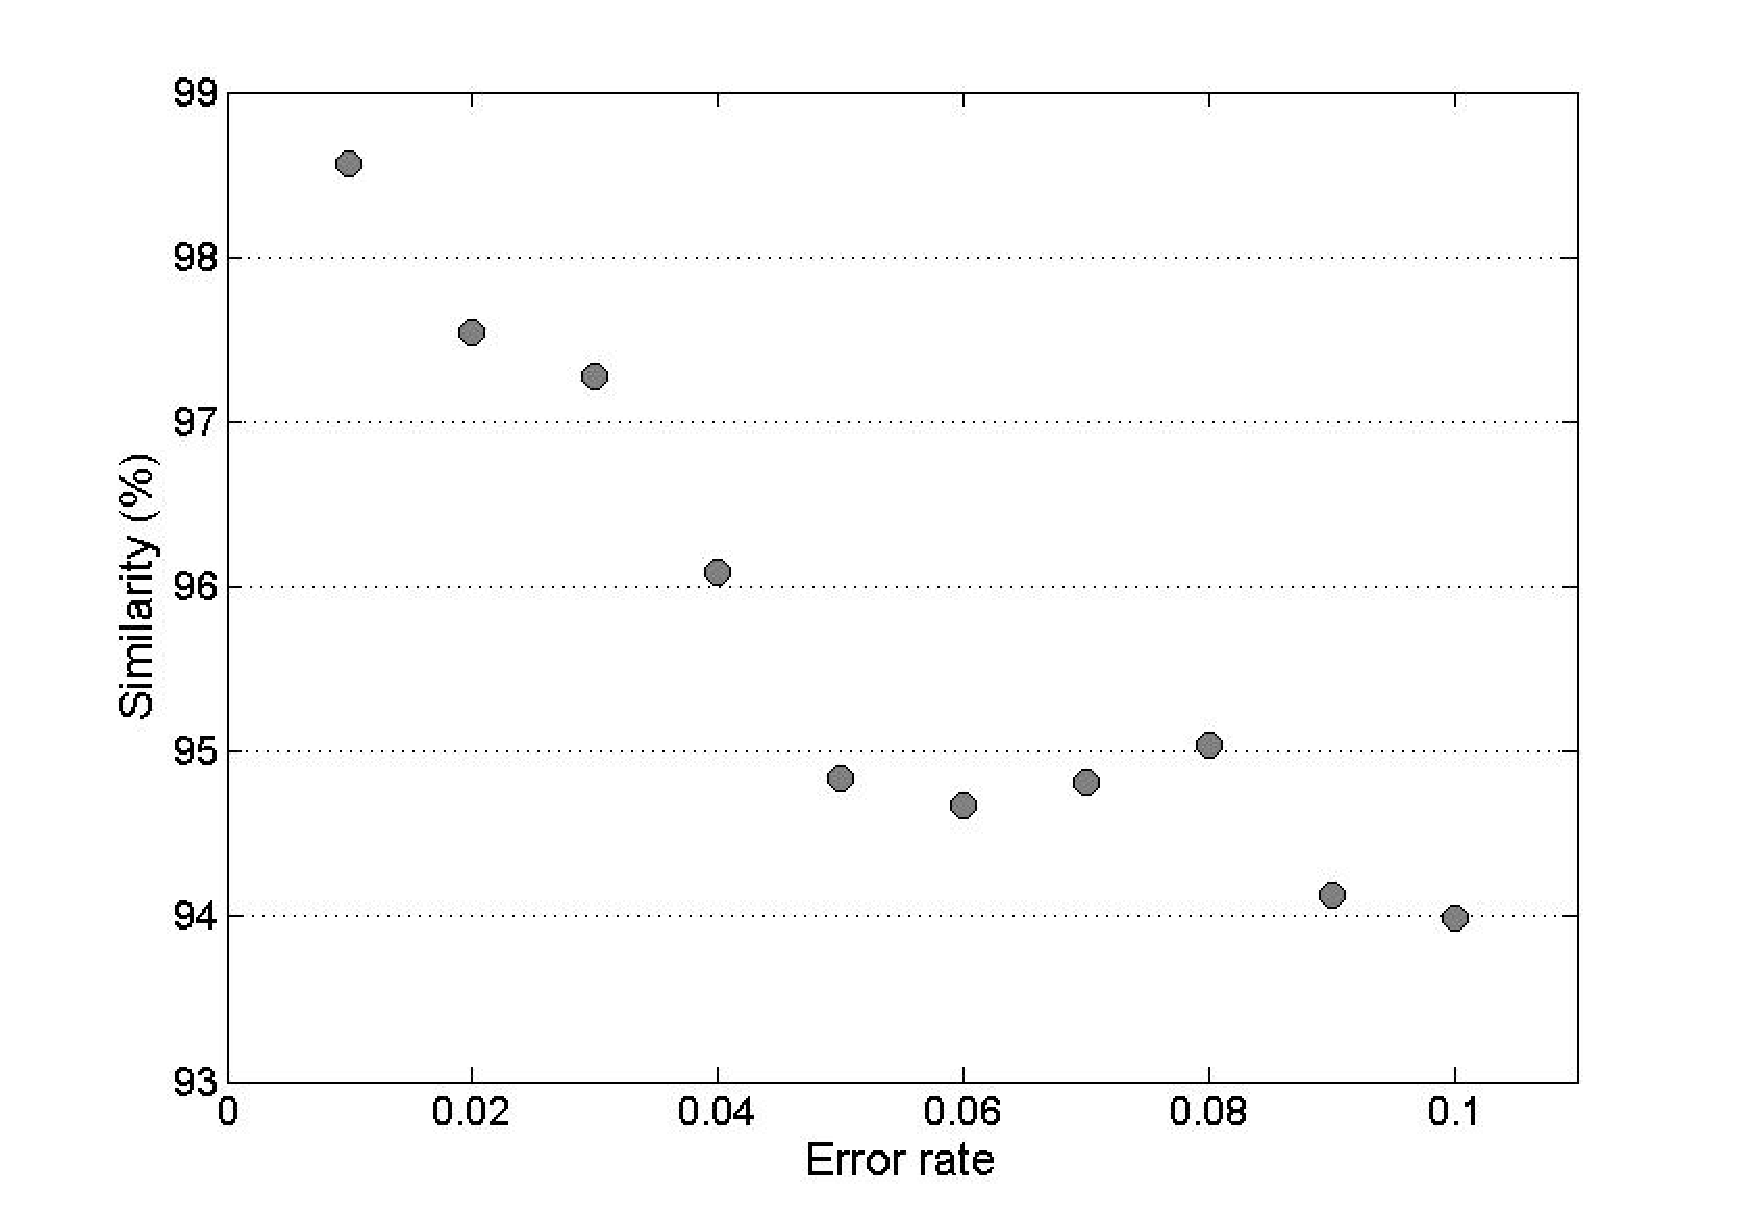
\includegraphics[width=0.6\textwidth]{./figs/error_correction.pdf}
  \caption{Error Tolerance for the Comparison Engine \cite{hu2012cmos}}
  \label{fig:err}
\end{figure}

